\chapter{Planificación}

Para realizar este proyecto, lo he dividido en varias etapas. La primera etapa consta de definición del problema, búsqueda de objetivos e investigación del estado del arte (el cual ha sido abordado en los capítulo 1, 2 y 3 de este documento). La segunda etapa consistirá en un aprovisionamiento de la infraestructura necesaria para los tests del software o de los modelos predictivos. La tercera etapa consistirá en implementación y experimentación de los modelos predictivos usando uno o varios frameworks de Machine Learning o Deep Learning. Y por último, una cuarta etapa de implementación, despliegue y monitorización de un microservicio básico y la realización de los tests de infraestructura necesarios.\\

La metodología que usaré para llevar a cabo el proyecto será \textit{Kanban} \cite{kanban}. Esta metodología usa las llamadas \textit{Historias de Usuario} para reflejar los deseos de los clientes, las cuales tengo en \textit{GitHub} enunciadas en los \textit{issues} de este proyecto \cite{issues}. Además de lo anterior, en esta metodología se utiliza un tablero que nos permite visualizar el flujo del trabajo. En este tablero se encuentran las tareas necesarias en tres columnas distintas: \textit{To do} (aún no se ha empezado), \textit{In progress} (se está realizando ahora mismo) y \textit{Done} (finalizada).\\

Además de los anterior, \textit{GitHub} también nos permite agrupas las \textit{issues} en \textit{milestones}, cada milestone representará una etapa de este proyecto y haré uno especial para las Historias de Usuario y otro para documentación. Y si lo de antes es poco, también nos permite añadir un tablero \textit{kanban} al repositorio. En la Figura \ref{fig:kanban} se puede observar el que yo he realizado.\\

Podemos ver que \textit{GitHub} es una gran herramienta para el desarrollo de software que nos permite trabajar cómodamente de forma individual o en grupos.

\begin{figure}[H]
	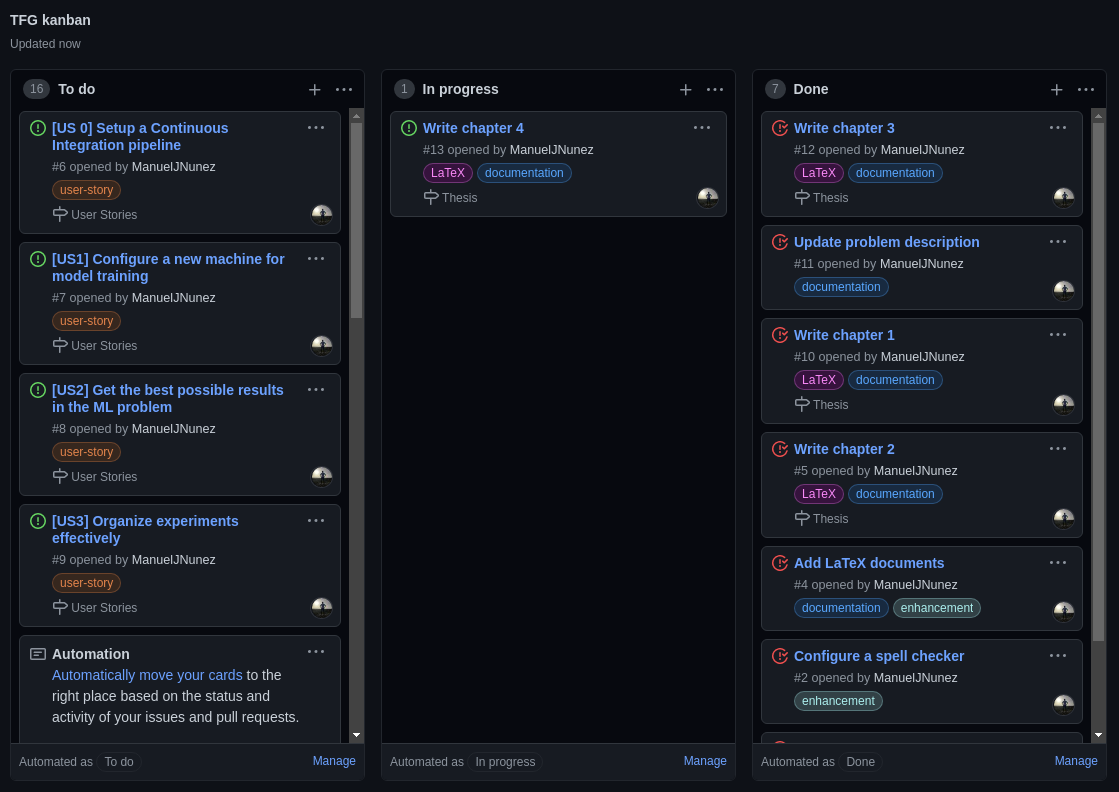
\includegraphics[scale=0.3]{imagenes/04_Planificacion/kanban.png}
	\centering
	\caption{Tablero \textit{kanban} en \textit{GitHub}. \cite{mykanban}}
	\label{fig:kanban}
\end{figure}
